\documentclass[12pt,letterpaper]{report}
\usepackage[margin=1in]{geometry}
\usepackage{graphicx}
\usepackage{amsmath}
\usepackage[font=small,labelfont=bf]{caption}
\usepackage[justification=centering]{caption}
\usepackage{tikz}
\usepackage{circuitikz}
\usepackage{siunitx}
\usepackage{float}
\newlength \figwidth
\setlength \figwidth {0.75\linewidth}

\begin{document}

\title{E153 Laboratory Assignment \#8}
\author{Courtney Keeler and Stephen Pinto\\
Harvey Mudd College}
\date{November 20, 2013}
\maketitle

\section*{List of Materials}
\begin{itemize}
	\item Tektronix 2212 Oscilloscope
	\item Pomona 4550B (10X probe)
	\item Elenco LCM-1950 Multimeter
	\item NE 555 IC
	\item 2N3904 transistor
	\item Standard resistors
	\item Standard capacitors
\end{itemize}

\section*{Purpose}
The purpose of this lab is to develop the formula for the oscillation frequency of a square wave oscillator circuit based on the charge and discharge time of the capacitor.

\section*{Procedure}

\begin{enumerate}
\item Build the circuit shown in Figure \ref{fig:circuit}
\item Measure the output and confirm that the frequency is correctly predicted by Equation \ref{eq:frequency}
\item Look at the waveform on the capacitor and record the voltage levels between which it runs
\item Make a prediction about what will be seen on the capacitor when $R_B$ is replaced with a short circuit
\item Make a prediction about what will be seen at the output when $R_B$ is replaced with a short circuit
\item Replace $R_B$ with a short circuit and compare the capacitor and output waveforms to those predicted 
\item Derive the formula for the oscillator frequency using the charge and discharge time of the capacitor
\end{enumerate}

\begin{figure}
\centering
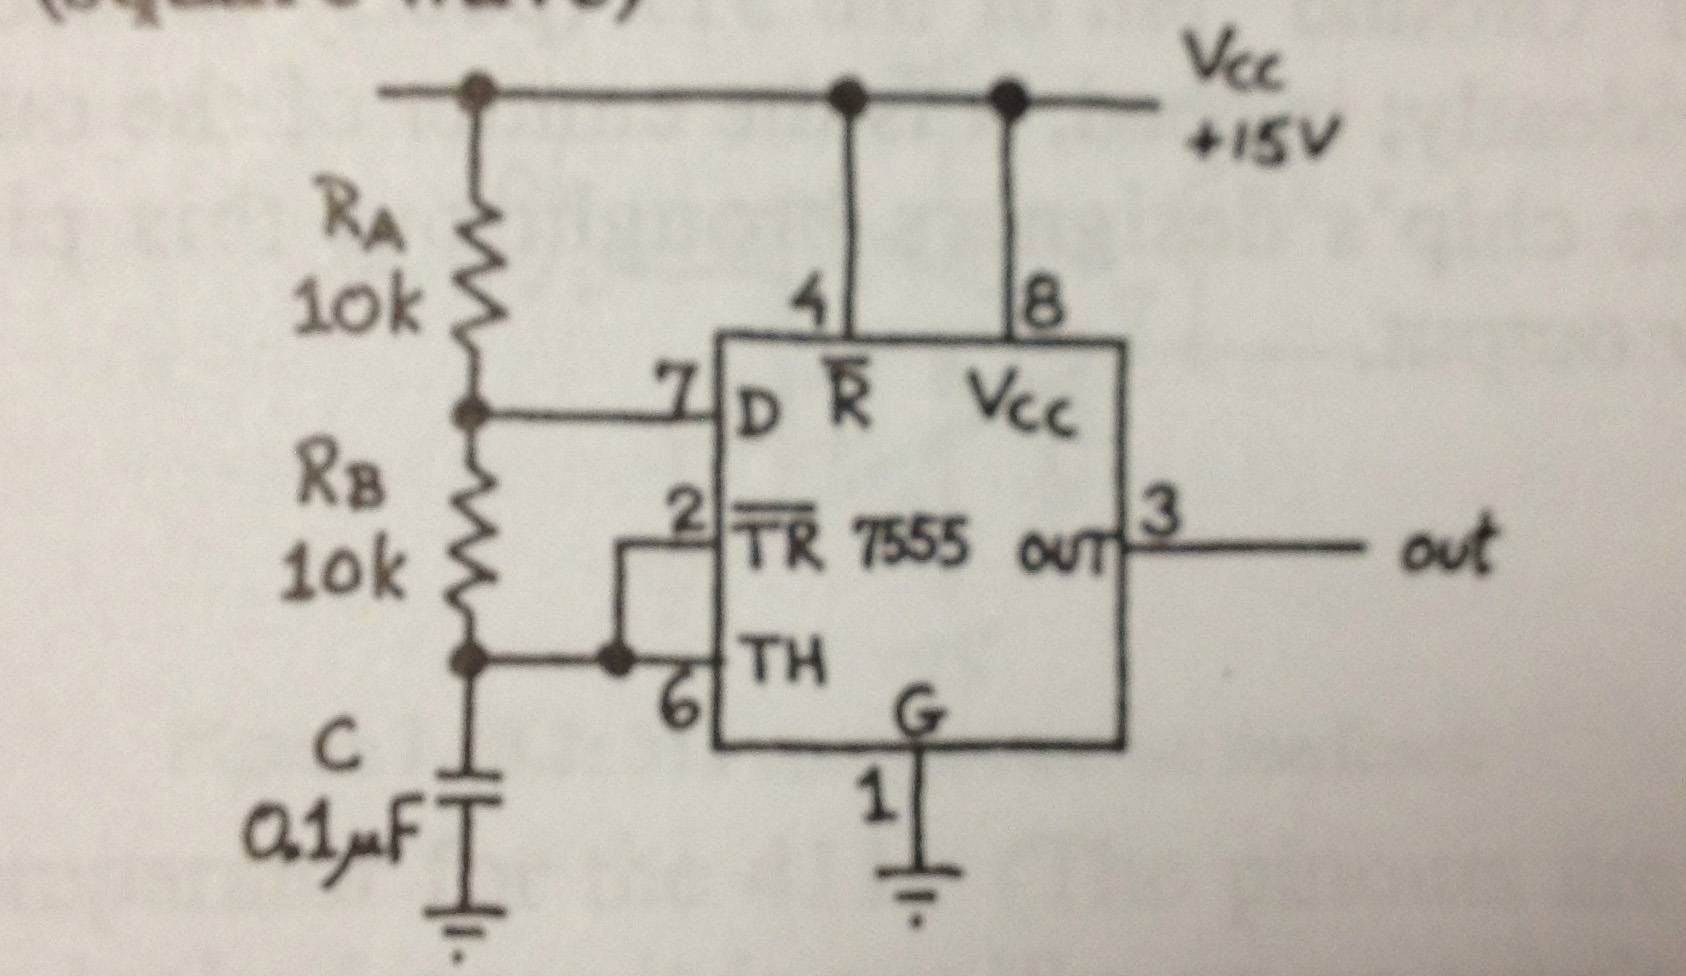
\includegraphics[width=\figwidth, keepaspectratio=true]{lab8_images/circuit.jpg}
\caption{Circuit diagram of the square wave oscillator.}
\label{fig:circuit}
\end{figure}

\begin{equation} \label{eq:frequency}
f_{osc}=\frac{1}{0.7(R_A + 2R_B)C}
\end{equation}

\section*{Results}

Actual values:
\begin{itemize}
\item $R_A$ = 9.82 k$\Omega$
\item $R_B$ = 9.9 k$\Omega$
\item C = 99.5 nF
\end{itemize}

We can calculate the expected frequency with the given equation:

$$
f_{osc} = \frac{1}{0.7(9.82\text{x}10^3 + 2\text{ x }9.9\text{x}10^3)99.5\text{x}10^{-9}} = 484.7 \text{ Hz.}
$$
Figure \ref{fig:output} shows the output waveform of the square wave oscillator. While we expected a frequency close to 500 Hz, we observed a frequency output of only 400 Hz.

\begin{figure}[H]
\centering
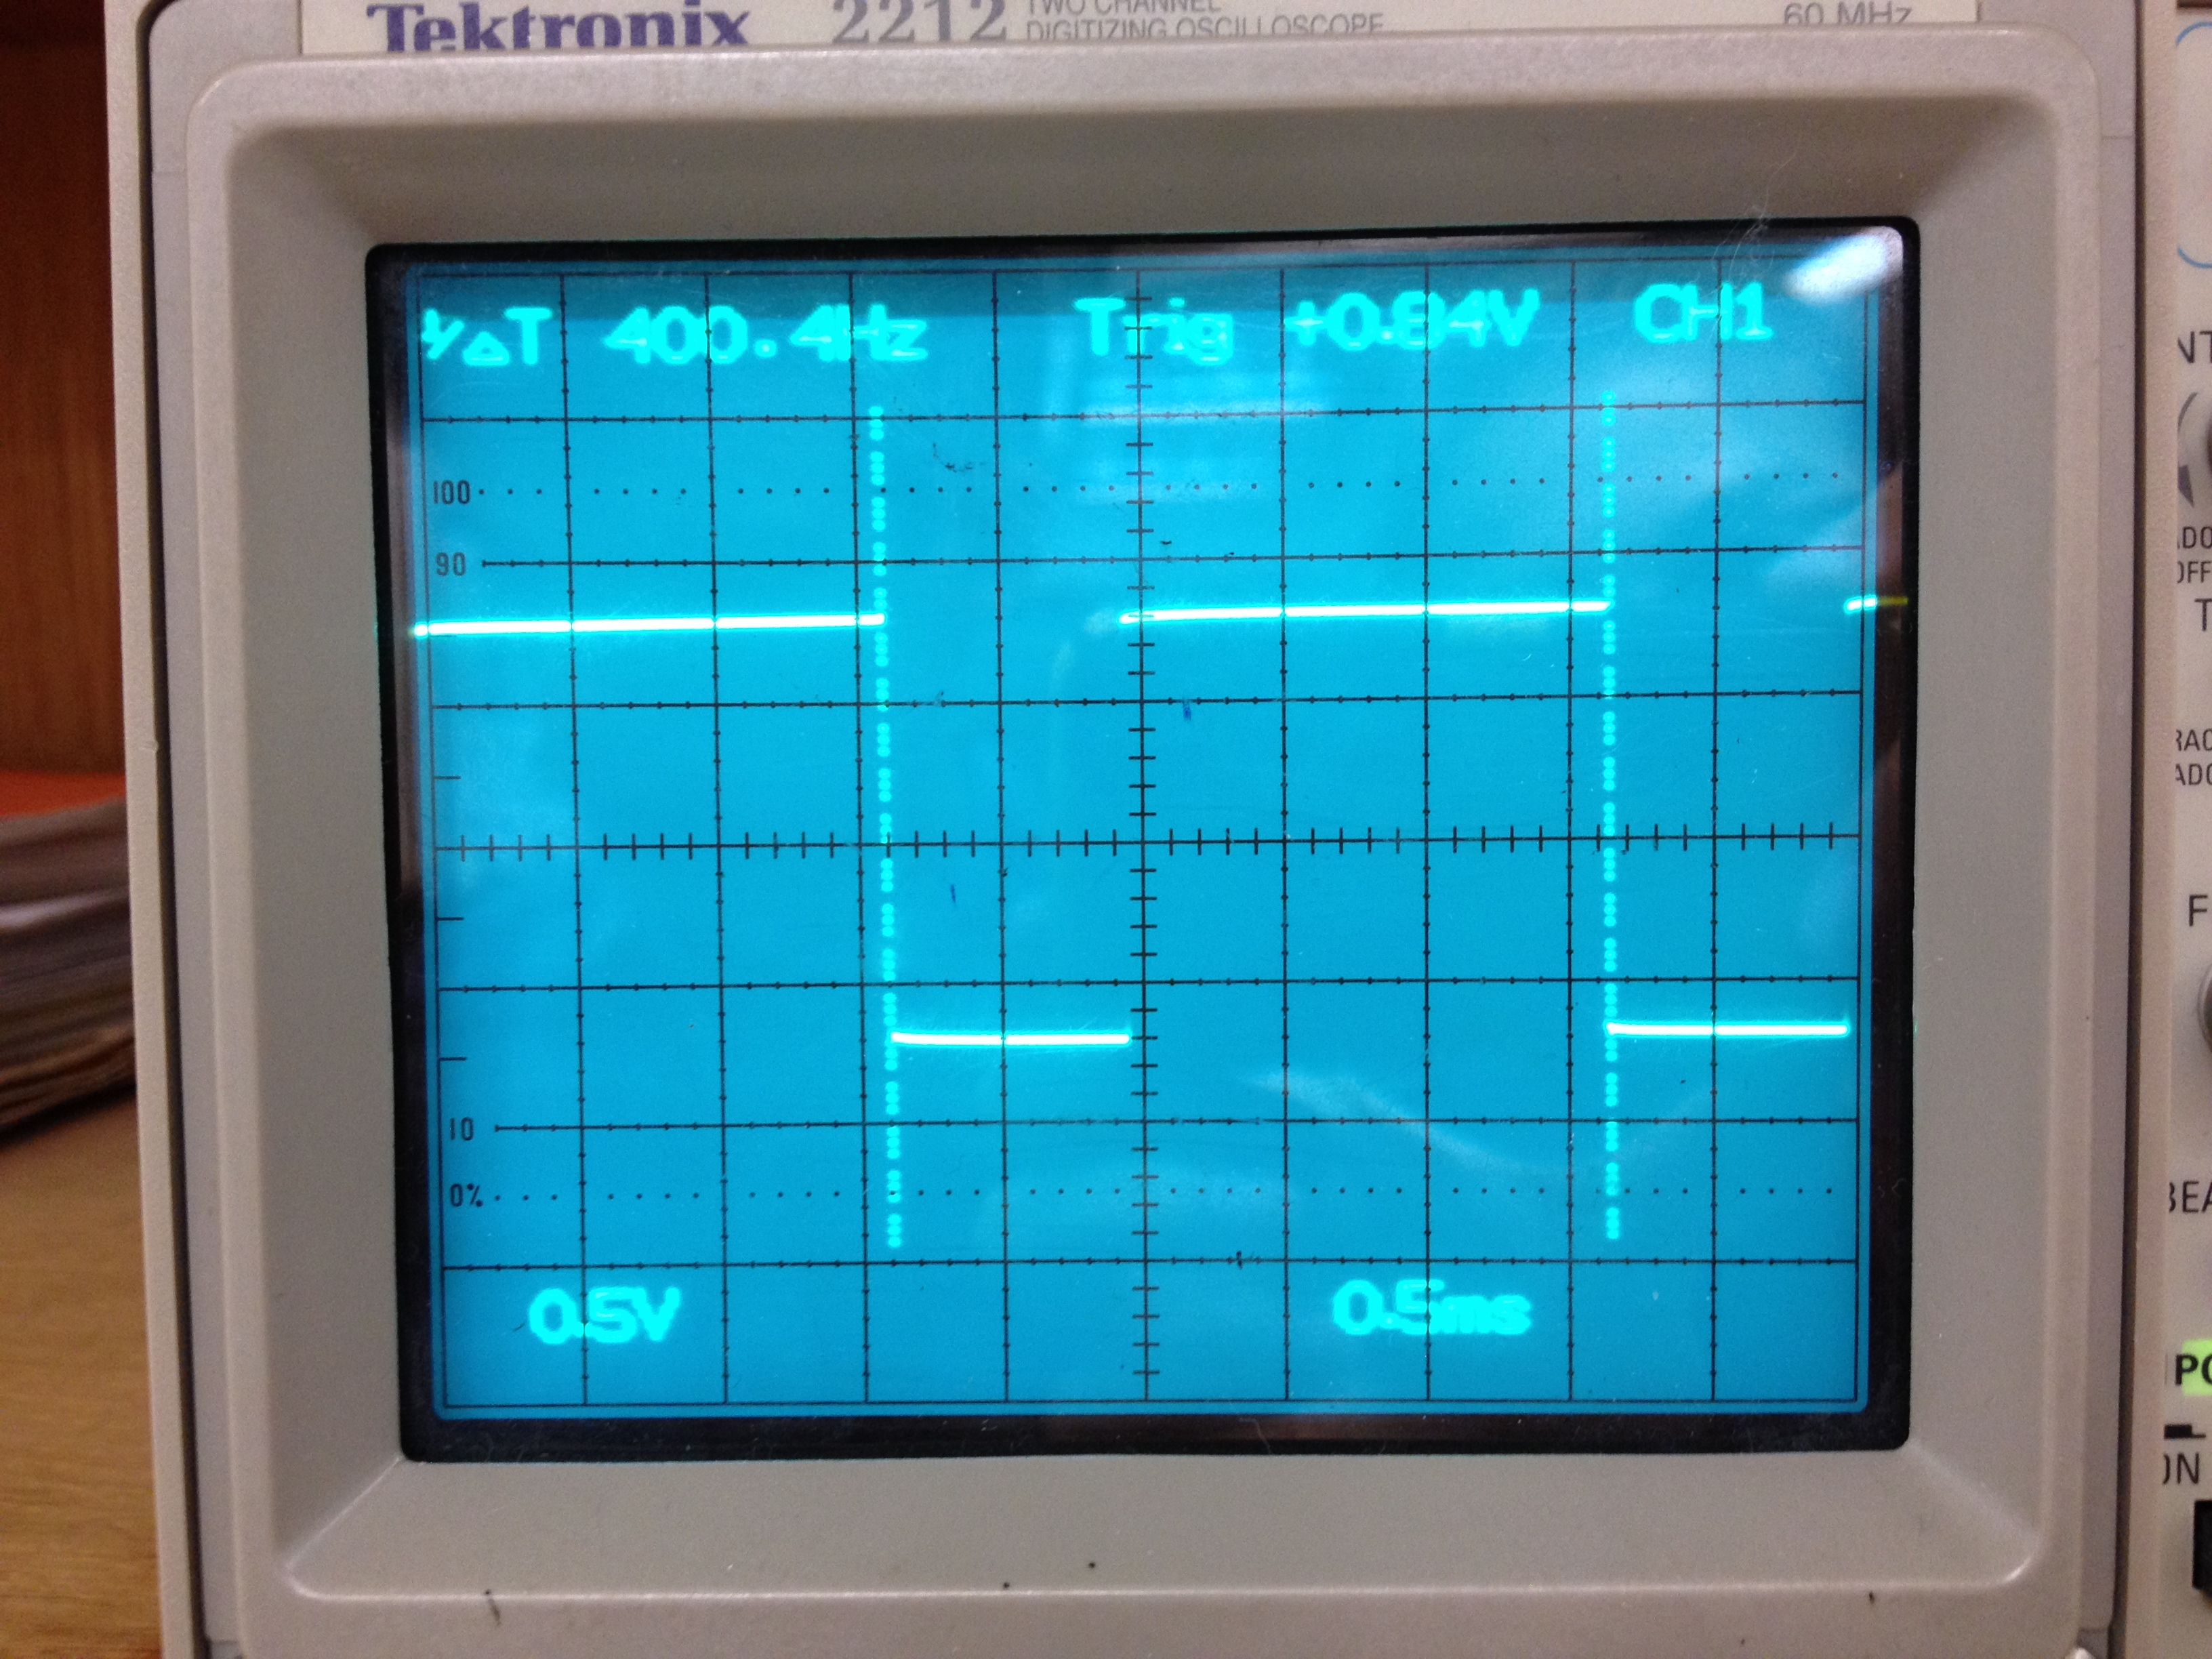
\includegraphics[width=\figwidth, keepaspectratio=true]{lab8_images/output.jpg}
\caption{Output waveform of the square wave oscillator circuit.}
\label{fig:output}
\end{figure}

Figure \ref{fig:cap} shows the voltage across the capactior of the square wave oscillator circuit. The voltage varies between 

\begin{figure}[H]
\centering
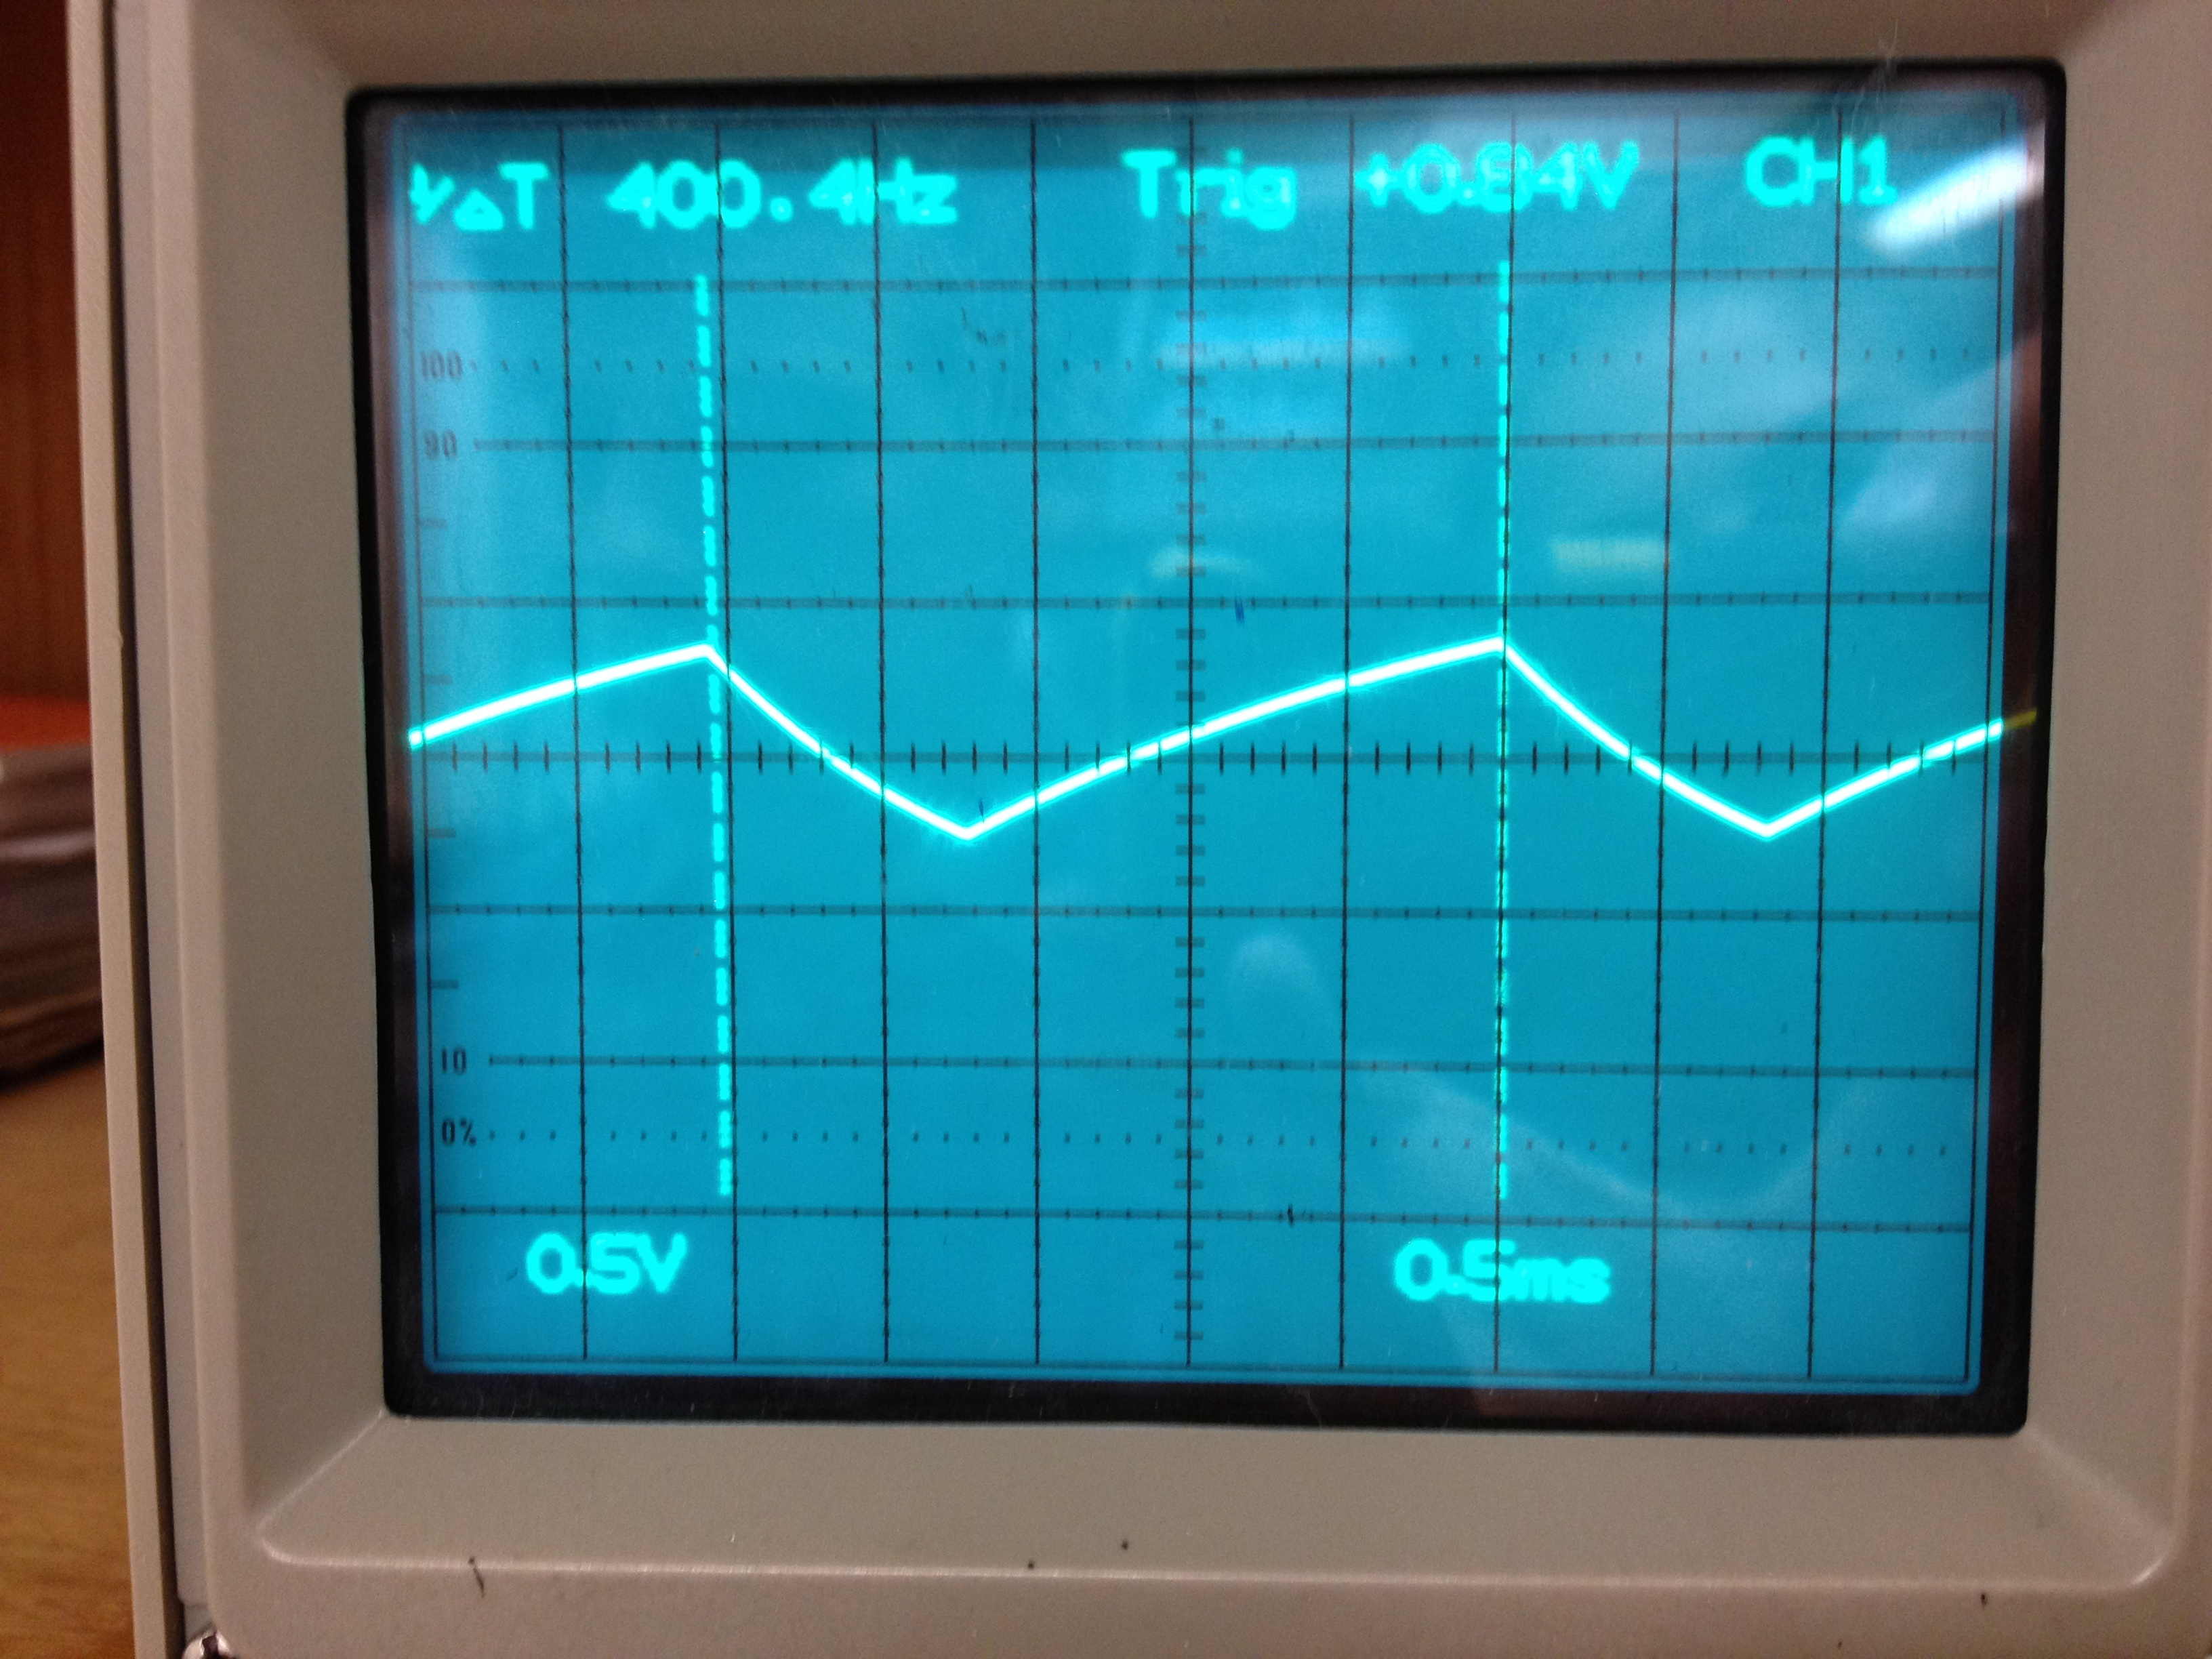
\includegraphics[width=\figwidth, keepaspectratio=true]{lab8_images/cap.jpg}
\caption{Waveform across the capacitor of the square wave oscillator circuit.}
\label{fig:cap}
\end{figure}

If $R_B$ were to be shorted, the discharge time to ground for the capacitor would become instantaneous. This means the capacitor is always charging because once it hits $\frac{2V_{CC}}{3}$, it will immediately discharge and begin charging again. This means the output is always high, or is essentially a square wave with duty cycle = 1. Figure \ref{fig:short} confirms this. 

\begin{figure}[H]
\centering
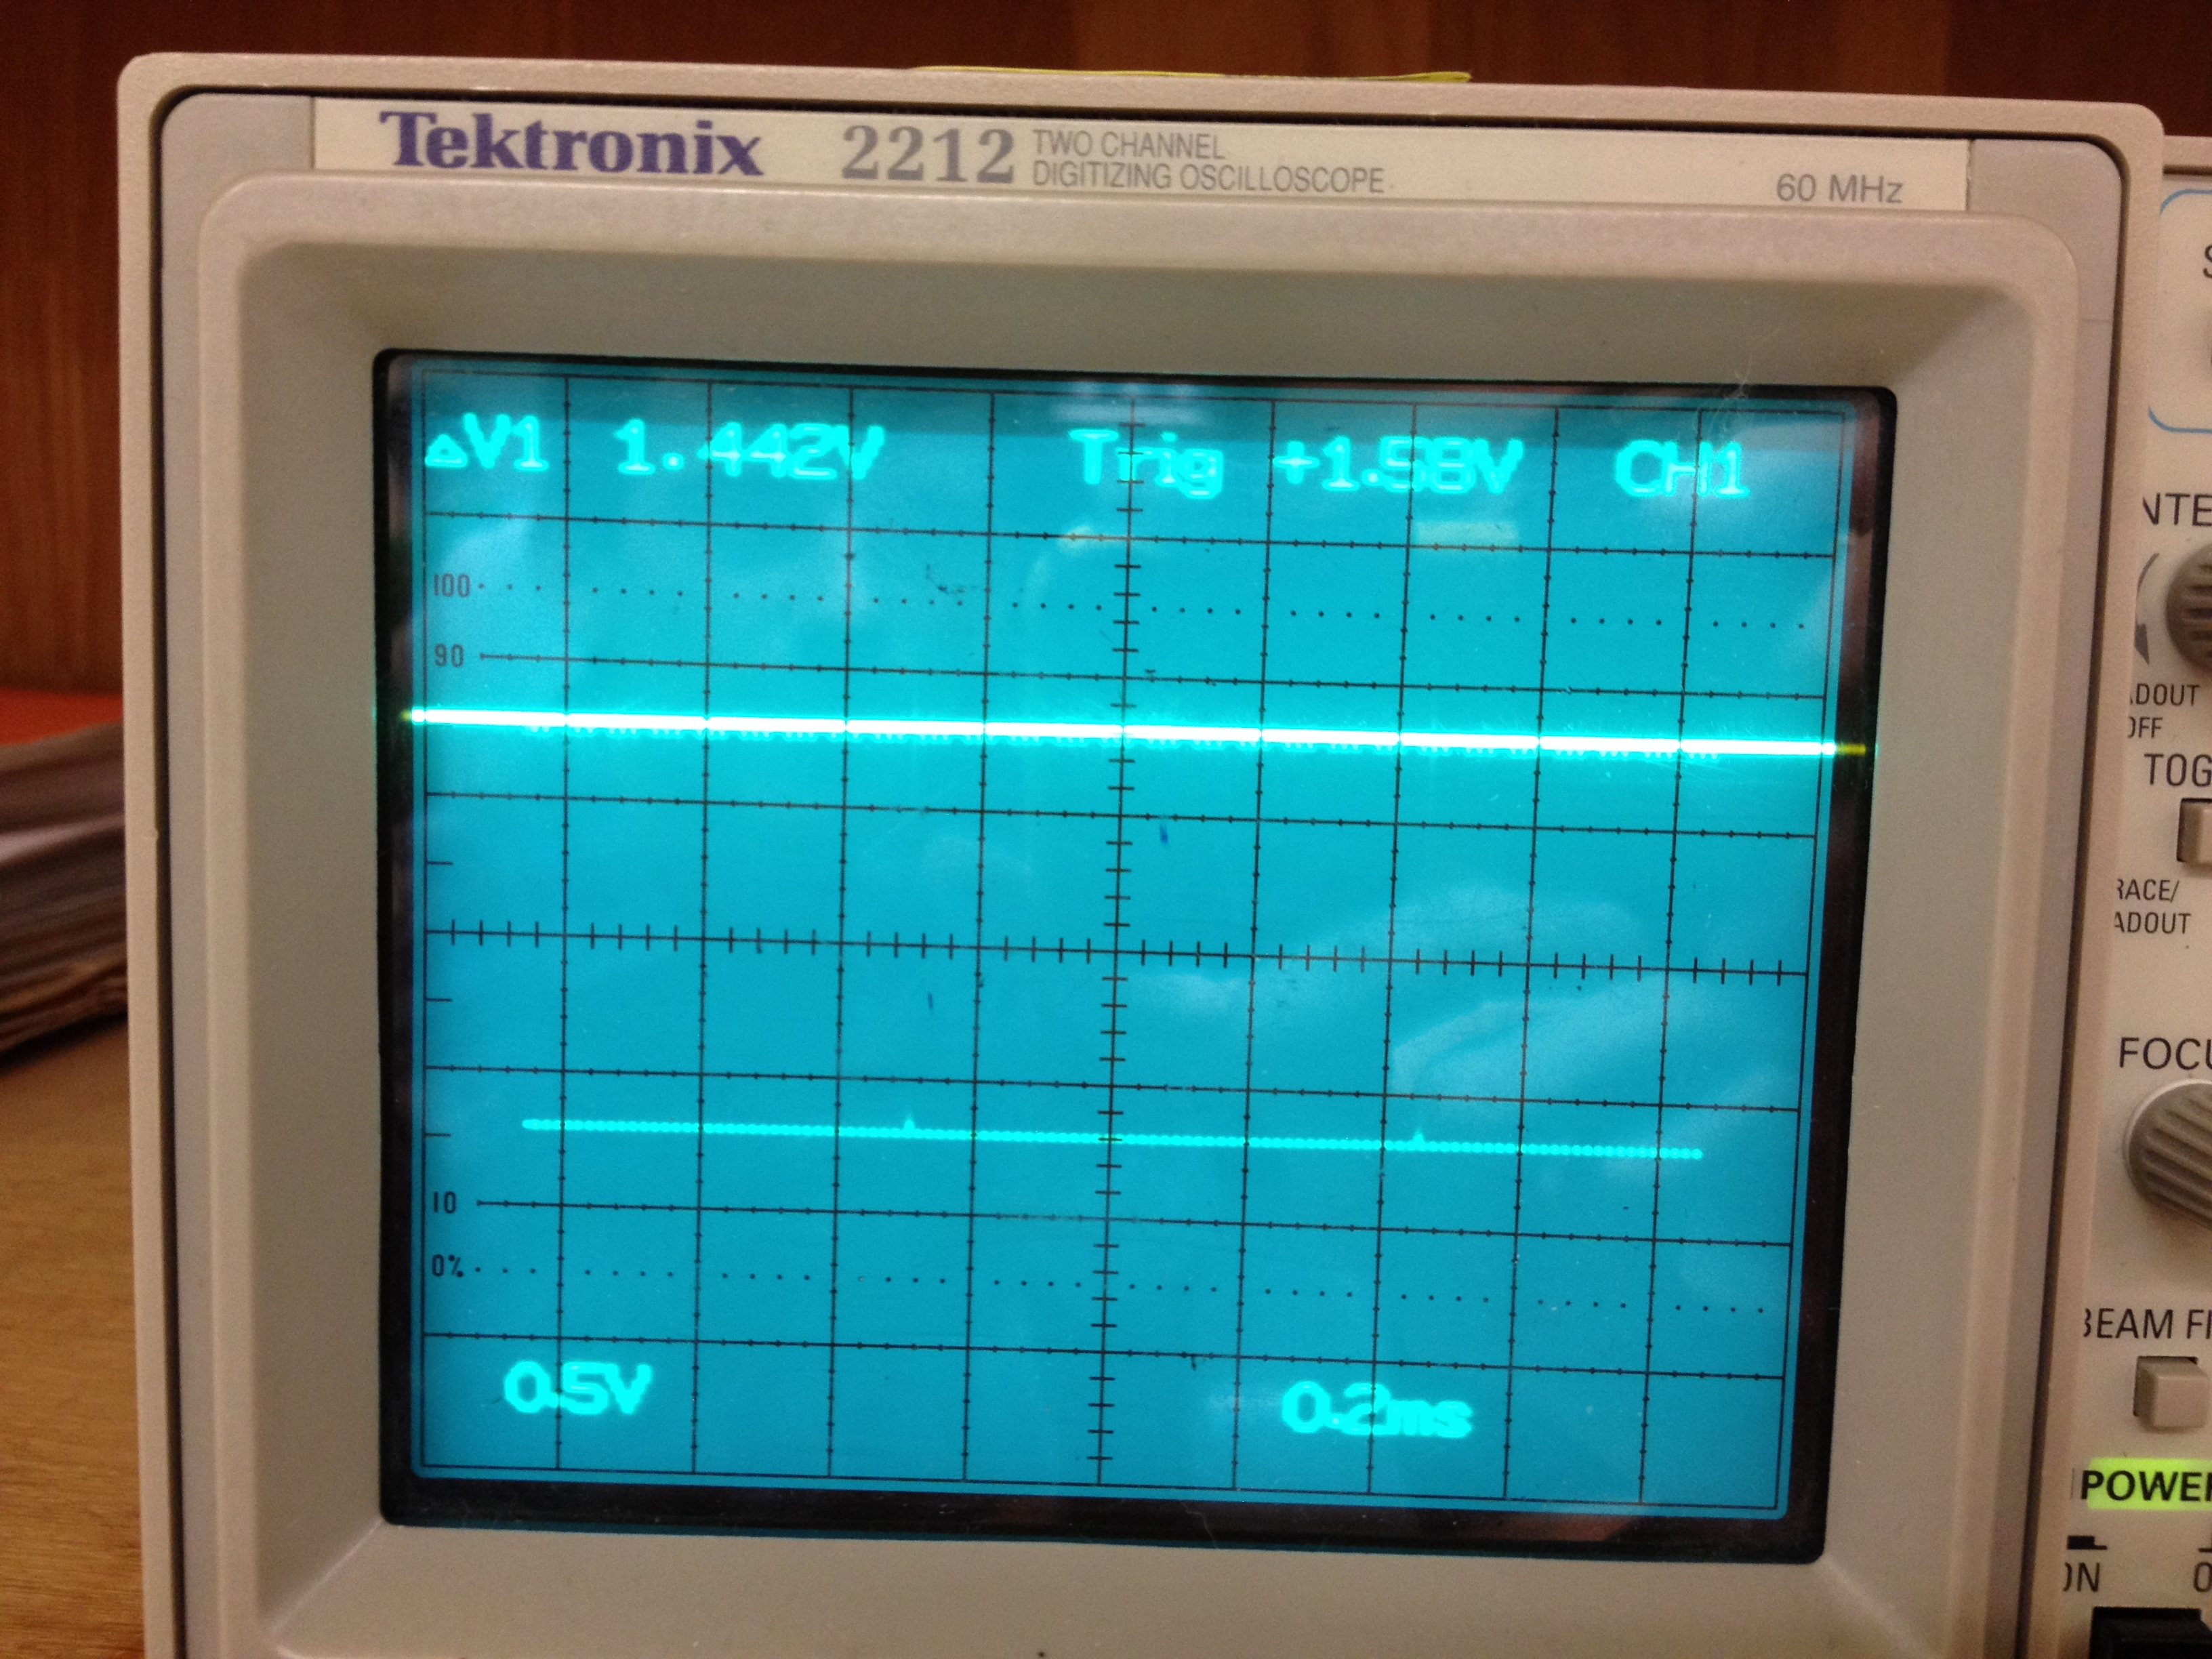
\includegraphics[width=\figwidth, keepaspectratio=true]{lab8_images/shorted.jpg}
\caption{Output waveform of the square wave oscillator circuit with resistor $R_B$ shorted.}
\label{fig:short}
\end{figure}

\section*{$T_{osc}$ Derivation}
The charging and discharging equations of a capacitor and resistor in series are, respectively,

$$
V_C = V_{CC}(1-e^{\frac{-t}{\tau}})
$$

$$
V_C = V_{CC}e^{\frac{-t}{\tau}}
$$

where $\tau = RC$. So a capacitor charging to $\frac{1V_{CC}}{3}$ will take

$$
t_{1/3} = -\tau \ln (1 - \frac{1}{3}) = -\tau \ln (\frac{2}{3})
$$

and one charging to $\frac{2V_{CC}}{3}$ will take

$$
t_{2/3} = -\tau \ln (1 - \frac{2}{3}) = -\tau_{\text{charge}} \ln (\frac{1}{3}).
$$

Thus a capacitor charging from $\frac{1V_{CC}}{3}$ to $\frac{2V_{CC}}{3}$ will take

$$
t_{\text{charge}} = t_{2/3} - t_{1/3} = \tau_{\text{charge}} \ln (2).
$$

Making a similar argument for discharging from $\frac{2V_{CC}}{3}$ to $\frac{1V_{CC}}{3}$ yields

$$
t_{\text{discharge}} = \tau_{\text{discharge}} \ln (2).
$$

The total period is the sum of the two,

$$
T = t_{\text{discharge}} + t_{\text{charge}} = \ln (2) (\tau_{\text{discharge}} + \tau_{\text{charge}}).
$$

While the capacitor is charging up to $V_{CC}$, it is in series with $R_B$ and $R_A$. However, while the capacitor is discharging to ground, it is only in series with $R_B$ as the current will flow through $Q_1$, the discharge transistor, after going through $R_B$. Thus, the oscillation period is

$$
T = \ln (2) (R_A + 2 R_B) C.
$$

\section*{Conclusion}

In conclusion, this lab has shown that it is possible to derive a formula for the oscillation frequency of a square wace oscillator circuit based on only the charge and discharge time of the capacitor. It was also predicted and proven that shorting the resistor $R_B$ results in a square wave with a duty cycle of 1. The purpose of this lab, therefore, was met.

\end{document}

%photo 

%\begin{table}[ht]
%\caption{Voltage across each "diode"} % title of Table
%\centering 
%    \begin{tabular}{| c | c |} 
%    \hline
%    $V_{\text{BC}}$ & 0.711 V \\
%    $V_{\text{BE}}$ & 0.717 V \\
%    \hline
%    \end{tabular}
%    \label{table:section_1}
%\end{table}
